\documentclass{article}
\usepackage[utf8]{inputenc}

\title{SML - Exercise 2}
\author{Maximilian Nothnagel, Stefanie Martin}
\date{}

\usepackage{pythonhighlight}
\usepackage{graphicx}
\usepackage{amsmath}
\usepackage[font=small,labelfont=bf]{caption}

\begin{document}
	
	\maketitle
	
	\section{Task 1: Optimization}
	\subsection{1a) Numerical Optimization}
		\begin{python}
		#Function for calculating f'(x)
		def solveDerivative(x):
		#Calculate Derivative f'(x)
		result = 400 * math.pow(x, 3) + (2-400*(x+1)) * x-2 
		#print('f\'(', x,') =', result) #print result
		return result
		
		n = 20
		#needs to be surprisingly small for decent results. 
		learningRate = 0.000001 
		#Randomly determine starting x
		curX = random.randint(1, n-1) 
		for curIteration in range(1, 10000):
		curResult = solveDerivative(curX) 
		print(curIteration, " : f\'(", curX,") =", curResult)
		#negate to always move towards negative
		diff = learningRate * -curResult 
		#apply to curX for next iteration
		curX += diff 
		if curIteration % 2000 == 0: 
		input("Press Enter to continue...")
		
		print("final X is", curX, "; with f'(",curX,")= ", solveDerivative(curX) )	
		\end{python}
	Learning rate impacts the size of the "steps" we take in each iteration. Since we are approximating, we generally step over the lowest point at some point, and then start stepping back and forth over the lowest point. \\
	A smaller learning rate will lead to smaller steps while moving towards the lowest point, but to a larger gap created by stepping back and forth over the lowest point once it has been found.\\
	Larger learning rates lead to fast, unaccurate conclusions, smaller rarely come to a conclusion within 10k iterations.\\
	Choose the learning rate just right to get a accurate conclusion, while still arriving at the conclusion in most cases.
	(conclusion meaning the lowest point)\\
	Samples taken from one running of the script: \\
		\begin{align*}
			\#0001 & f'(18,0) = 2196034,0\\
			\#1000 & f'( 1,8132) = 345,853\\
			\#2000 & f'( 1,6567) = 59,694\\
			\#3000 & f'( 1,6262) = 13,164\\
			\#4000 & f'( 1,6193) = 3,050\\
			\#5000 & f'( 1,6177) = 0,715\\
			\#6000 & f'( 1,6173) = 0,1679\\
			\#7000 & f'( 1,61721) = 0,0395\\
			\#8000 & f'( 1,617187) = 0,00923\\
			\#9000 & f'( 1,61718799) = 0,0021822\\
			\#10000 & f'(1,6171806) = 0,0005131
		\end{align*}
	\begin{minipage}{0.9\linewidth}
		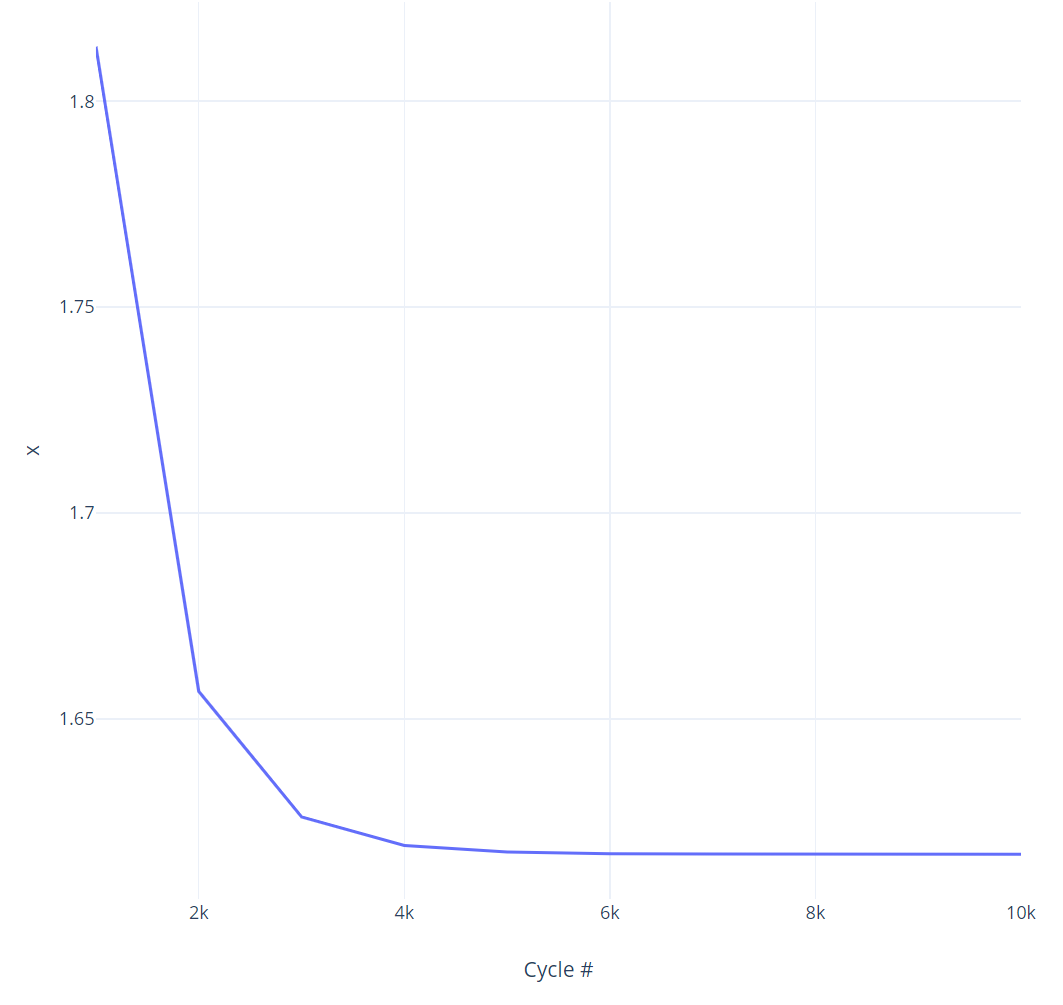
\includegraphics[width=1\textwidth]{Graph1.png}
		\captionof{figure}{Graph for f'(x) throughout the cycles.}
	\end{minipage}\\
	Cycle \#1 excluded for scaling. We can observe a rapid descent of the gradient, slowing down as it approaches 0

\subsection{1b) Gradient Descent Variants}
\subsubsection{1)}
	% https://stats.stackexchange.com/questions/49528/batch-gradient-descent-versus-stochastic-gradient-descent
	% https://en.wikipedia.org/wiki/Gradient_descent#:~:text=Gradient%20descent%20is%20a%20first,the%20direction%20of%20steepest%20descent
	% https://towardsdatascience.com/batch-mini-batch-stochastic-gradient-descent-7a62ecba642a
	Batch Gradient Descent: From a random starting point, move toward the direction of lowest gradient a distance based on the Gradient. Repeat. Very accurate, but computationally expensive.\\
	Stochastic Gradient Descent: From a random starting point, pick a random point P2 in the sorrounding. move roughly towards P2, following the direction of the lowest Gradient. Repeat. This reduces the computing in each step, opting instead for random generation. \\
	%Mini-Batch habe ich nicht so ganz verstanden
	Mini-Batch Gradient Descent: Create Mini-Batch of datapoints out of the whole set. Compute mean gradient for the Mini-batch, use it in selecting for the next Mini-Batch. Repeat. Saves Memory, by only ever working on small parts of the dataset.
	
\subsubsection{2)}
	Momentum is the idea of taking greater or smaller steps based on the results of each step. This is easily recognized in Batch/Vanilla Gradient Descent, and also present in the other variants.
	
\section{Task 2: Density Estimation - MLE}
\subsection{2a) Maximization Likelihood Estimate of the Exponential Distribution}
	Using Python we computed the maximum propabilities of the given function for x=[0..100] and s=[-40..40]\\
	$\frac{1}{s} * e^{-\frac{x}{s} }$		\\
	\begin{align*}
	Maximum of s= &-40 : & -0.025\\
	Maximum of s= &-20 : & -0.05\\
	Maximum of s= &-15 : & -0.06666666666666667\\
	Maximum of s= &-10 : & -0.1\\
	Maximum of s= &-5 :  &-0.2\\
	Maximum of s= &-4 :  &-0.25\\
	Maximum of s= &-3 :  &-0.3333333333333333\\
	Maximum of s= &-2 :  &-0.5\\
	Maximum of s= &-1 :  &-1.0\\
	Maximum of s= &0.01 : & -100.0\\
	Maximum of s= &0 :  &Undefined\\
	Maximum of s= &0.01 :&  100.0\\
	Maximum of s= &1 :  &1.0\\
	Maximum of s= &2 :  &0.5\\
	Maximum of s= &3 :  &0.3333333333333333\\
	Maximum of s= &4 :  &0.25\\
	Maximum of s= &5 :  &0.2\\
	Maximum of s= &10 :  &0.1\\
	Maximum of s= &15 :  &0.06666666666666667\\
	Maximum of s= &20 :  &0.05\\
	Maximum of s= &40 :  &0.025\\
	\end{align*}
	When s converges towards 0, the likelihood rises to infinity.\\
	When s rises towards $\pm\infty$ , the likelihood approaches 0
	
\section{Task 3: Density Estimation}
\subsection{3a) Prior Probabilities}
Putting the data into a python script and averaging out the classes yields the following priors: \\
C1 averaged: $-0.7750366930281244$ \\
C2 averaged: $12.627232147035425$

\subsection{3b) Biased ML Estimate}
An estimator's bias describes a tendency of the estimates to differ from the parameter being estimated in a consistent way.

\end{document}